%!TEX root = ../thesis.tex

\section{背景}
近年,人手不足を背景にサービスロボットの需要が高まり,日常生活の中で目にする機会が増えている.現在,実用化に至っているサービスロボットは,館内の案内\cite{AYUDA:online},警備\cite{SQ-2:online},掃除\cite{Pana:online},配膳\cite{BellaBot:online},など,1つの作業に特化したロボットが主流である.一方で,複数の作業が行えるサービスロボットであるモバイルマニピュレータロボットの開発が進められている.モバイルマニピュレータロボットは,自律移動ロボットにマニピュレータを搭載したロボットであり,PAL Robotics社のTIAGo(図\ref{fig:TIAGo}参照) やトヨタ自動車のHSR(図\ref{fig:HSR}参照) などが代表例として挙げられる.これらのロボットは,人に代わって様々な作業ができる汎用的なサービスロボットとして実用化が期待されている\cite{古賀達也201937_707}.本研究では,オフィス環境で活動するモバイルマニピュレータロボットを「オフィスロボット」と定義して研究を進める.

オフィスロボットは様々な企業や研究室で開発が進められているものの,設計データを公開している例が少なく,オープンプラットフォームが不足している.オープンプラットフォームとして設計データを公開することは,利用者によるハードウェアの改良を容易にし,開発者間の技術交流を促進する点で大きな利点がある.例えば,自律移動ロボットのオープンソースハードウェアである i-Cart シリーズは,本研究室で開発されている orne-box をはじめとする様々なロボットのベースとして活用されてきた.このようにハードウェアプラットフォームが整備されている場合には,開発者はハードウェア製作の工数を削減し,ソフトウェア開発やタスク実装に注力できる.さらに,開発者間の知識や成果を共有することで,技術発展が加速すると考えられる.

そこで本研究では,オープンプラットフォームオフィスロボットの開発を行う.特に本項では,オフィスロボットの要となるアームに着目し,そのメカニズムの設計と製作について述べる.

\begin{figure}[h]
  \centering
  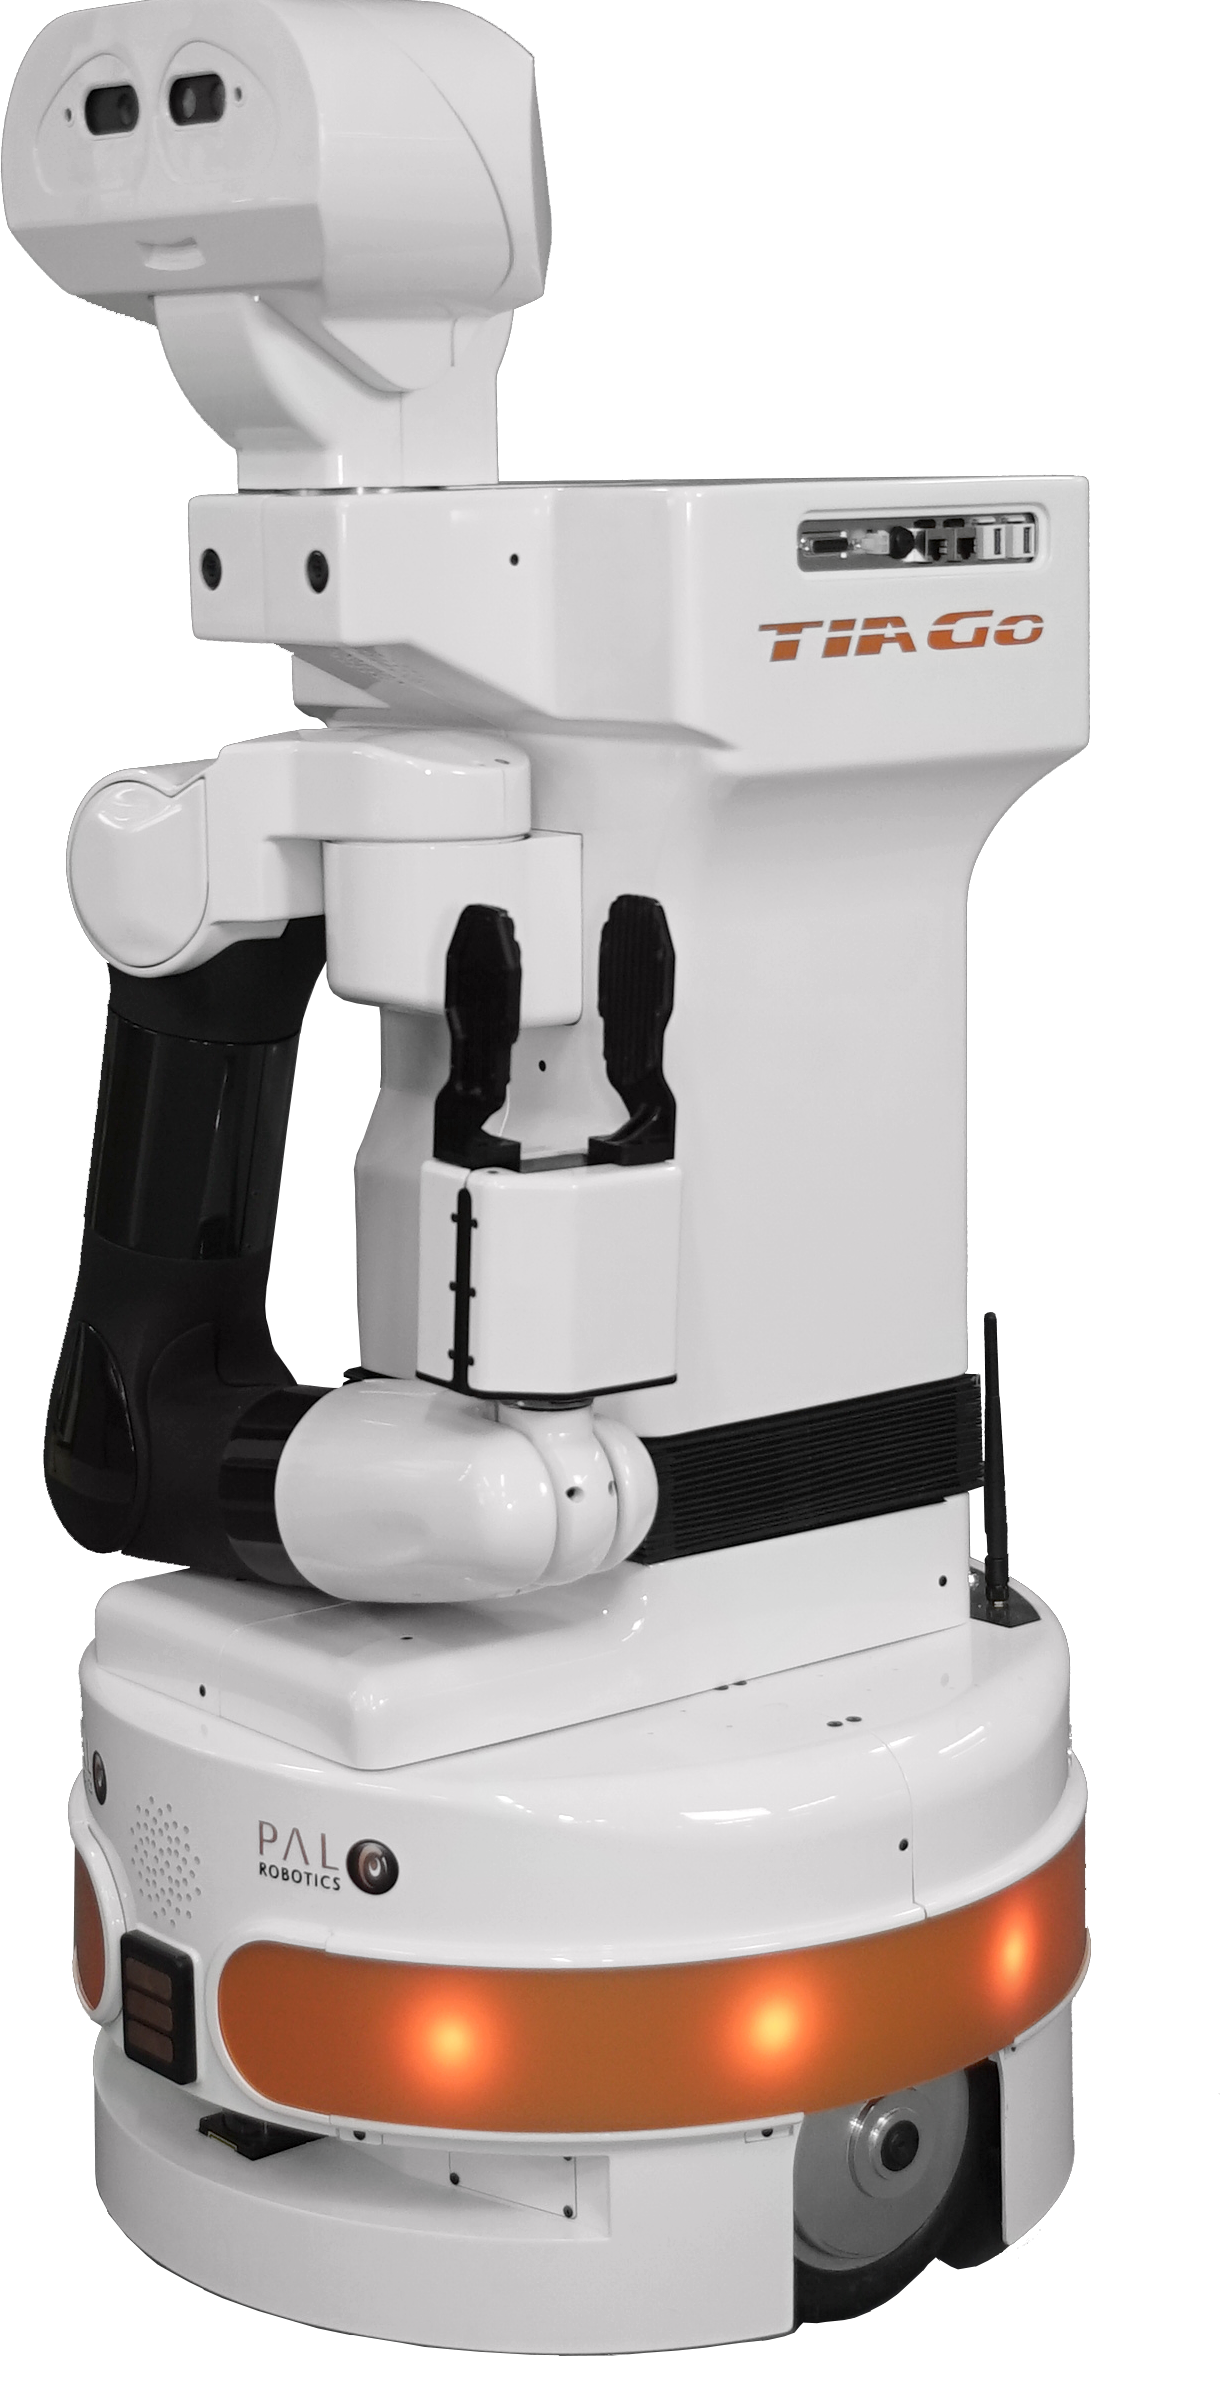
\includegraphics[width=25mm]{images/png/TIAGo.png}
  \caption[TIAGo from PAL-Robotics]{TIAGo from PAL-Robotics (source: \cite{TIAGo:online})}
  \label{fig:TIAGo}
\end{figure}
\begin{figure}[h]
  \centering
  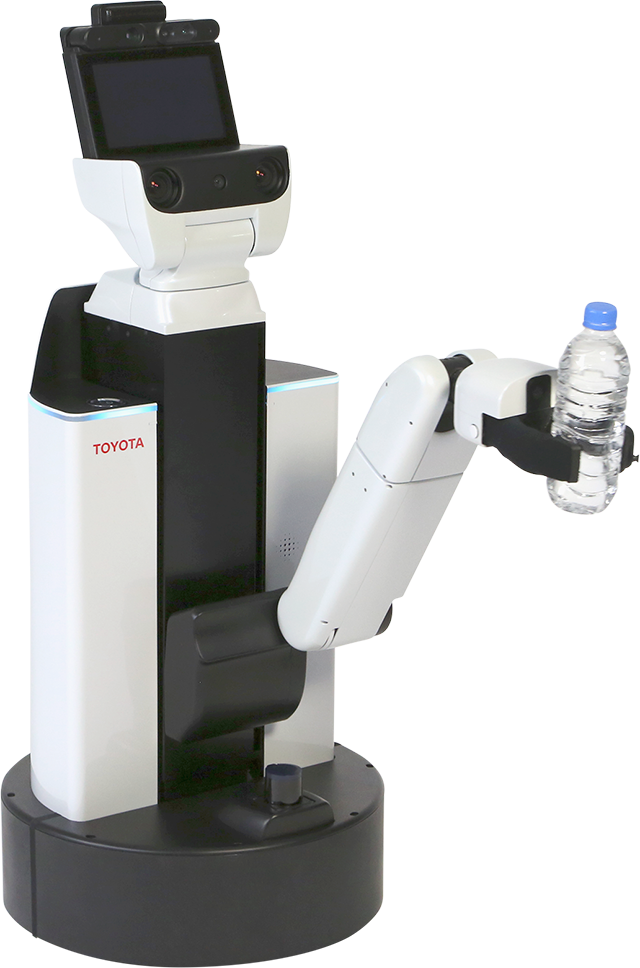
\includegraphics[width=25mm]{images/png/HSR.png}
  \caption[HSR from TOYOTA]{HSR from TOYOTA (source: \cite{HSR:online})}
  \label{fig:HSR}
\end{figure}

\newpage